\documentclass{standalone}

\usepackage{tikz}
\usepackage{amssymb}
\usetikzlibrary{calc, positioning}
\begin{document}
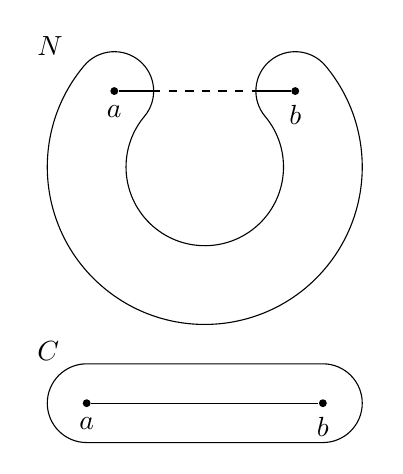
\begin{tikzpicture}
	\def\region[#1][#2]{
	\path[#1]
	let
	\n1 = {#2},
	\n2 = {#2-180},
	\n3 = {#2+180},
	in
	(-\n1:1) arc[start angle = -\n1, end angle = \n2, radius = 1] coordinate (1)
	arc[start angle = \n1, end angle = \n3, radius = 0.5] coordinate (2)
	arc[start angle = \n2, end angle = -\n1, radius = 2] coordinate (3)
	arc[start angle = -\n1, end angle = -\n2, radius = 0.5] coordinate (4)
	-- cycle;
	}

	\region[draw][-40];
	\node[circle, fill, minimum size = 0.1cm, inner sep = 0, label=below:{$ a $}]
	(a) at ($ 1/2*(1) + 1/2*(2) $){};
	\node[circle, fill, minimum size = 0.1cm, inner sep = 0, label=below:{$ b $}]
	(b) at ($ 1/2*(3) + 1/2*(4) $){};
	\draw[dashed] (a) -- (b);

	\begin{scope}
		\region[clip][-40];
		\draw (a) -- (b);
	\end{scope}

	\begin{scope}[yshift=-3cm]
		\draw (-1.5,0.5) -- (1.5,0.5)
		arc[start angle = 90, end angle = -90, radius = 0.5]
		-- (-1.5,-0.5)
		arc[start angle = 270, end angle = 90, radius = 0.5]
		-- cycle;
		\node[circle, fill, minimum size = 0.1cm, inner sep = 0, label=below:{$ a $}]
		(a) at (-1.5,0){};
		\node[circle, fill, minimum size = 0.1cm, inner sep = 0, label=below:{$ b $}]
		(b) at (1.5,0){};
		\draw (a) -- (b);
	\end{scope}

	\node[right] at (current bounding box.north west) {$ N $};
	\node[right] at ($(current bounding box.south west) + (0,1.2)$) {$ C $};

\end{tikzpicture}
\end{document}
